\subsection*{a}
Figure \ref{fig:MC} is a graph representation of Markov chain.\\
\begin{figure}[h!]
	\centering
	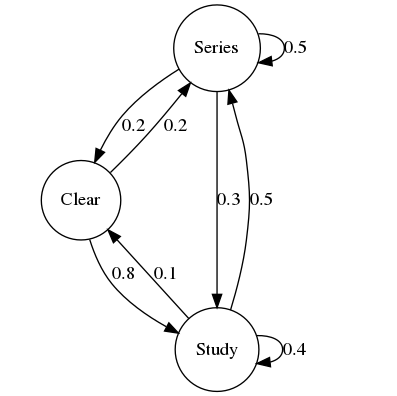
\includegraphics[width=0.5\linewidth]{task5-graph.png}
	\caption{Markov-chain graph}
	\label{fig:MC}
\end{figure}\\
The corresponding probability matrix is $Q = 
\begin{pmatrix}
	0.4 & 0.5 & 0.1 \\
	0.3 & 0.5 & 0.2 \\
	0.8 & 0.2 & 0
\end{pmatrix}
$
where rows and columns represent in order of [Study, Series, Clear]
\subsection*{b}
As soon as student is currently done clearing $p_0 = [0, 0, 1]$. To find probability distribution after 2 steps
$p_2 = p_0\cdot Q^2 = [0.38, 0.5, 0.12]$. 
\subsection*{c}
As soon, as matrix is connected and aperiodic $lim_{t\to \infty}p_t = \pi$. After 8 iterations:
\begin{verbatim}
input matrix:
[0.4,0.5,0.1]
[0.3,0.5,0.2]
[0.8,0.2,  0]
p0:[0.4164,0.1955,0.3881]
p1:[ 0.5357, 0.3836,0.08073]
p2:[0.3939,0.4758,0.1303]
p3:[0.4045,0.4609,0.1345]
p4:[0.4077,0.4596,0.1326]
p5:[0.4071,0.4602,0.1327]
p6:[0.4071,0.4602,0.1328]
p7:[0.4071,0.4602,0.1327]
p8:[0.4071,0.4602,0.1327]
\end{verbatim}
distribution converges to $p_8 = [0.4071,0.4602,0.1327]$. Thus the fraction of time, that student spends in long term is $0.4071$.